%%%%%%%%%%%%%%
%% Run LaTeX on this file several times to get Table of Contents,
%% cross-references, and citations.

%% If you have font problems, you may edit the w-bookps.sty file
%% to customize the font names to match those on your system.

%% w-bksamp.tex. Current Version: Feb 16, 2012
%%%%%%%%%%%%%%%%%%%%%%%%%%%%%%%%%%%%%%%%%%%%%%%%%%%%%%%%%%%%%%%%
%
%  Sample file for
%  Wiley Book Style, Design No.: SD 001B, 7x10
%  Wiley Book Style, Design No.: SD 004B, 6x9
%
%
%  Prepared by Amy Hendrickson, TeXnology Inc.
%  http://www.texnology.com
%%%%%%%%%%%%%%%%%%%%%%%%%%%%%%%%%%%%%%%%%%%%%%%%%%%%%%%%%%%%%%%%

%%%%%%%%%%%%%
% 7x10
%\documentclass{wileySev}

% 6x9

\documentclass{wileysix}
\UseRawInputEncoding
\usepackage{graphicx}
\usepackage{tabularx}
\usepackage{listings}
\usepackage{paralist}
\usepackage{gensymb}
\usepackage{float}

\usepackage{color}
 
\definecolor{codegreen}{rgb}{0,0.6,0}
\definecolor{codegray}{rgb}{0.5,0.5,0.5}
\definecolor{codepurple}{rgb}{0.58,0,0.82}
\definecolor{backcolour}{rgb}{0.95,0.95,0.92}
 
\lstdefinestyle{mystyle}{
    backgroundcolor=\color{backcolour},   
    commentstyle=\color{codegreen},
    keywordstyle=\color{magenta},
    numberstyle=\tiny\color{codegray},
    stringstyle=\color{codepurple},
    basicstyle=\footnotesize,
    breakatwhitespace=false,         
    breaklines=true,                 
    captionpos=b,                    
    keepspaces=true,                 
    numbers=left,                    
    numbersep=5pt,                  
    showspaces=false,                
    showstringspaces=false,
    showtabs=false,                  
    tabsize=2,
    language=sh
}
 
\lstset{style=mystyle}

%%%%%%%
%% for times math: However, this package disables bold math (!)
%% \mathbf{x} will still work, but you will not have bold math
%% in section heads or chapter titles. If you don't use math
%% in those environments, mathptmx might be a good choice.

% \usepackage{mathptmx}

% For PostScript text
\usepackage{w-bookps}

%%%%%%%%%%%%%%%%%%%%%%%%%%%%%%%%%%%%%%%%%%%%%%%%%%%%%%%%%%%%%%%%
%% Other packages you might want to use:

% for chapter bibliography made with BibTeX
% \usepackage{chapterbib}

% for multiple indices
% \usepackage{multind}

% for answers to problems
% \usepackage{answers}

%%%%%%%%%%%%%%%%%%%%%%%%%%%%%%
%% Change options here if you want:
%%
%% How many levels of section head would you like numbered?
%% 0= no section numbers, 1= section, 2= subsection, 3= subsubsection
%%==>>
\setcounter{secnumdepth}{3}

%% How many levels of section head would you like to appear in the
%% Table of Contents?
%% 0= chapter titles, 1= section titles, 2= subsection titles, 
%% 3= subsubsection titles.
%%==>>
\setcounter{tocdepth}{2}

%% Cropmarks? good for final page makeup
%% \docropmarks

%%%%%%%%%%%%%%%%%%%%%%%%%%%%%%
%
% DRAFT
%
% Uncomment to get double spacing between lines, current date and time
% printed at bottom of page.
% \draft
% (If you want to keep tables from becoming double spaced also uncomment
% this):
% \renewcommand{\arraystretch}{0.6}
%%%%%%%%%%%%%%%%%%%%%%%%%%%%%%

%%%%%%% Demo of section head containing sample macro:
%% To get a macro to expand correctly in a section head, with upper and
%% lower case math, put the definition and set the box 
%% before \begin{document}, so that when it appears in the 
%% table of contents it will also work:

\newcommand{\VT}[1]{\ensuremath{{V_{T#1}}}}

%% use a box to expand the macro before we put it into the section head:

\newbox\sectsavebox
\setbox\sectsavebox=\hbox{\boldmath\VT{xyz}}

%%%%%%%%%%%%%%%%% End Demo


\begin{document}


\booktitle{\textsf{\huge Project Android Sederhana\\ Membuat Aplikasi Monitoring\\ Kinerja Berbasis GPS}}
\subtitle{}

\authors{M. Yusril H. S\\ Kadek Diva K. M.\\ Chandra Kirana P.\\
\affil{D4 Teknik Informatika, Politeknik Pos Indonesia}
%Floyd J. Fowler, Jr.\\
%\affil{University of New Mexico}
}

\offprintinfo{Project Android Sederhana Membuat Aplikasi Monitoring Kinerja Berbasis GPS}{M. Yusril H. S, Kadek Diva K. M., \& Chandra Kirana P.}

%% Can use \\ if title, and edition are too wide, ie,
%% \offprintinfo{Survey Methodology,\\ Second Edition}{Robert M. Groves}

%%%%%%%%%%%%%%%%%%%%%%%%%%%%%%
%% 
\halftitlepage

\titlepage


\begin{copyrightpage}{2020}
%Survey Methodology / Robert M. Groves . . . [et al.].
%\       p. cm.---(Wiley series in survey methodology)
%\    ``Wiley-Interscience."
%\    Includes bibliographical references and index.
%\    ISBN 0-471-48348-6 (pbk.)
%\    1. Surveys---Methodology.  2. Social 
%\  sciences---Research---Statistical methods.  I. Groves, Robert M.  II. %
%Series.\\
%
%HA31.2.S873 2007
%001.4'33---dc22                                             2004044064
\end{copyrightpage}

\dedication{`Jika Kamu tidak dapat menahan lelahnya belajar, 
Maka kamu harus sanggup menahan perihnya Kebodohan.'
~Imam Syafi'i~}

\begin{contributors}
\name{Rolly Maulana Awangga,} Informatics Research Center., Politeknik Pos Indonesia, Bandung,
Indonesia



\end{contributors}

\contentsinbrief
\tableofcontents
\listoffigures
\listoftables
\lstlistoflistings


\begin{foreword}
Sepatah kata dari Kaprodi, Kabag Kemahasiswaan dan Mahasiswa
\end{foreword}

\begin{preface}
Buku ini diciptakan bagi yang awam dengan pemrograman Android sekalipun.

\prefaceauthor{D. K. Murti \& C. K. Poetra}
\where{Bandung, Jawa Barat\\
Januari, 2020}
\end{preface}


\begin{acknowledgments}
Terima kasih atas semua masukan dari para rekan-rekan agar bisa membuat buku ini 
lebih baik dan lebih mudah dimengerti.

Terima kasih ini juga ditujukan khusus untuk team IRC yang 
telah fokus untuk belajar dan memahami bagaimana buku ini mendampingi proses 
Proyek 3.
\authorinitials{D. K. M. \& C. K. P.}
\end{acknowledgments}

\begin{acronyms}
\acro{ACGIH}{American Conference of Governmental Industrial Hygienists}
\acro{AEC}{Atomic Energy Commission}
\acro{OSHA}{Occupational Health and Safety Commission}
\acro{SAMA}{Scientific Apparatus Makers Association}
\end{acronyms}

\begin{glossary}
\term{git}Merupakan manajemen sumber kode yang dibuat oleh linus torvald.

\term{bash}Merupakan bahasa sistem operasi berbasiskan *NIX.

\term{linux}Sistem operasi berbasis sumber kode terbuka yang dibuat oleh Linus Torvald
\end{glossary}

\begin{symbols}
\term{A}Amplitude

\term{\hbox{\&}}Propositional logic symbol 

\term{a}Filter Coefficient

\bigskip

\term{\mathcal{B}}Number of Beats
\end{symbols}

\begin{introduction}

%% optional, but if you want to list author:

\introauthor{Rolly Maulana Awangga, S.T., M.T.}
{Informatics Research Center\\
Bandung, Jawa Barat, Indonesia}

Pada era disruptif  \index{disruptif}\index{disruptif!modern} 
saat ini. git merupakan sebuah kebutuhan dalam sebuah organisasi pengembangan perangkat lunak.
Buku ini diharapkan bisa menjadi penghantar para programmer, analis, IT Operation dan Project Manajer.
Dalam melakukan implementasi git pada diri dan organisasinya.

Rumusnya cuman sebagai contoh aja biar keren\cite{awangga2018sampeu}.

\begin{equation}
ABC {\cal DEF} \alpha\beta\Gamma\Delta\sum^{abc}_{def}
\end{equation}

\end{introduction}

%%%%%%%%%%%%%%%%%%Isi Buku_

\chapter{GPS}
\section{API}
Perintah navigasi direktori
\lstinputlisting{src/api/config.php}
\lstinputlisting{src/api/conn.php}

\lstinputlisting{src/api/mahasiswa/mahasiswa_login.php}
\lstinputlisting{src/api/mahasiswa/mahasiswa_registrasi.php}
\lstinputlisting{src/api/mahasiswa/mahasiswa_absensi.php}
\lstinputlisting{src/api/mahasiswa/mahasiswa_kegiatan.php}
\lstinputlisting{src/api/mahasiswa/mahasiswa_notifikasi.php}
\lstinputlisting{src/api/mahasiswa/mahasiswa_pembimbing.php}
\lstinputlisting{src/api/mahasiswa/mahasiswa_perusahaan.php}
\lstinputlisting{src/api/mahasiswa/mahasiswa_progress.php}
\lstinputlisting{src/api/mahasiswa/mahasiswa_progress_harian.php}
\lstinputlisting{src/api/mahasiswa/mahasiswa_ubah.php}
\lstinputlisting{src/api/mahasiswa/mahasiswa.php}

\lstinputlisting{src/api/dosen/dosen_login.php}
\lstinputlisting{src/api/dosen/dosen_mahasiswa.php}
\lstinputlisting{src/api/dosen/dosen_notifikasi.php}
\lstinputlisting{src/api/dosen/dosen_progress.php}
\lstinputlisting{src/api/dosen/dosen_progress_harian.php}
\lstinputlisting{src/api/dosen/dosen_ubah.php}
\lstinputlisting{src/api/dosen/dosen.php}


\chapter{Kebutuhan}
\section{Perintah Navigasi}
Perintah navigasi direktori


\chapter{Perancangan}
\section{Web}
Source code web
\lstinputlisting{src/web/config/config.php}
\lstinputlisting{src/web/config/database.php}

\lstinputlisting{src/web/controllers/ckelolauser.php}
\lstinputlisting{src/web/controllers/clogin.php}
\UseRawInputEncoding{src/web/controllers/cregister.php}
\lstinputlisting{src/web/controllers/dashboard.php}

\lstinputlisting{src/web/models/mdatapeta.php}
\lstinputlisting{src/web/models/mdatauser.php}
\lstinputlisting{src/web/models/mlogin.php}
\lstinputlisting{src/web/models/mregister.php}

\lstinputlisting{src/web/views/chartview.php}
\lstinputlisting{src/web/views/dosen.php}
\lstinputlisting{src/web/views/index.php}
\lstinputlisting{src/web/views/login.php}
\lstinputlisting{src/web/views/vgrafik.php}
\lstinputlisting{src/web/views/vkelolauser.php}
\lstinputlisting{src/web/views/vregister.php}



\chapter{Pengkodean}
\section{Persiapan dan pengenalan}
\subsection{Instalasi Java}
\subsection{Instalasi Android Studio}
\begin{enumerate}
	\item Kemudian klik dua kali pada installer yang telah di-download untuk memulai proses instalasi. Installer akan menampilkan Android Studio Setup seperti gambar berikut, lalu klik Next. 
	\begin{figure}[H]
		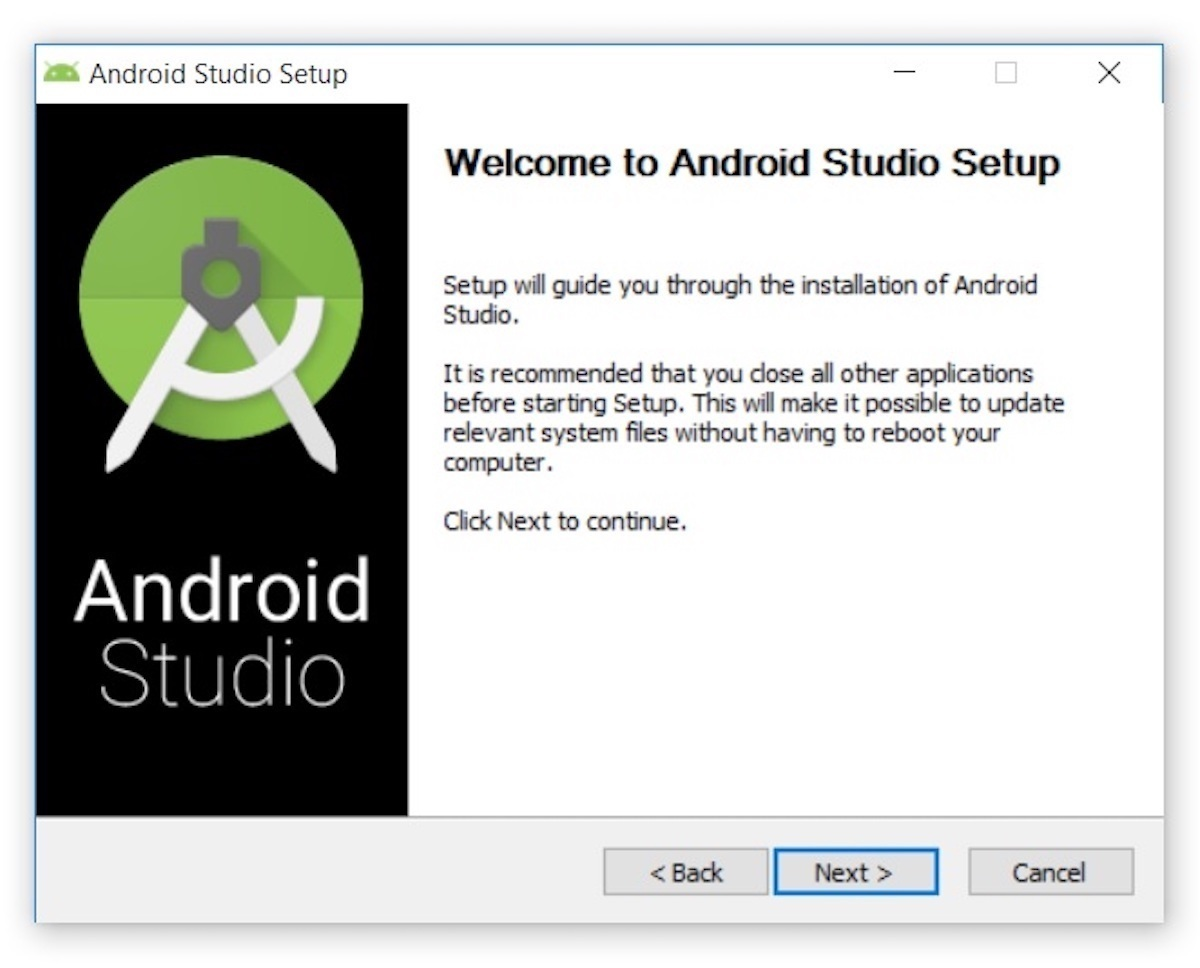
\includegraphics[width=4cm]{figures/installas/1.jpg}
		\centering
		\caption{Android Studio Setup.}
	\end{figure}
	\item Setelah itu kita diberi opsi untuk menginstal Android Virtual Device. Disini kita biarkan default setting-nya, lalu klik Next.
	\begin{figure}[H]
		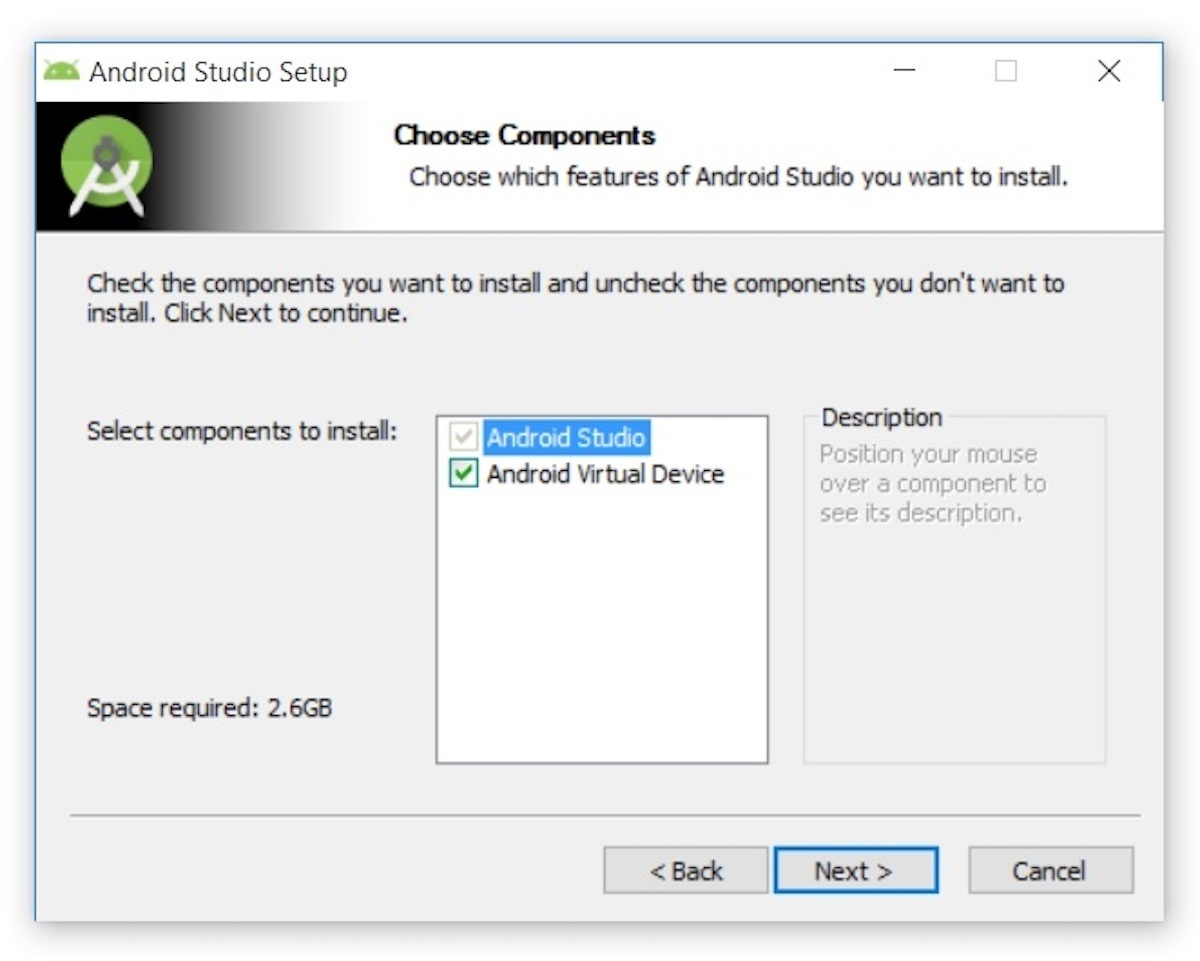
\includegraphics[width=4cm]{figures/installas/2.jpg}
		\centering
		\caption{Instal Android AVD.}
	\end{figure}
	\item Kemudian kita diminta untuk memilih lokasi tempat menginstal Android Studio-nya. Disini kita biarkan default setting-nya, lalu klik Next.
	\begin{figure}[H]
		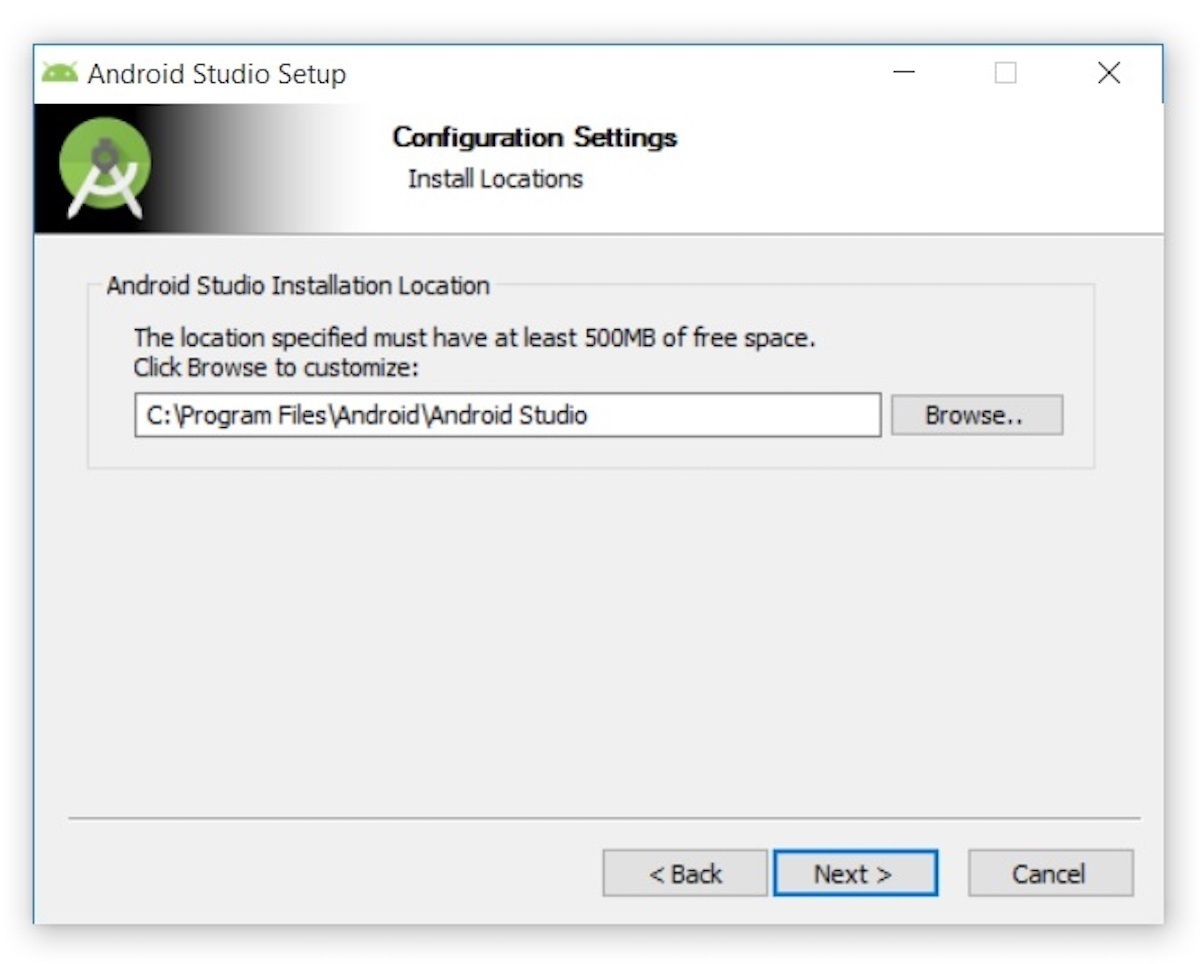
\includegraphics[width=4cm]{figures/installas/3.jpg}
		\centering
		\caption{Lokasi instal Android Studio.}
	\end{figure}
	\item Setelah itu, kita diberi opsi untuk membuat shortcut dari Android Studio. Disini kita biarkan default setting-nya, lalu klik Install.
	\begin{figure}[H]
		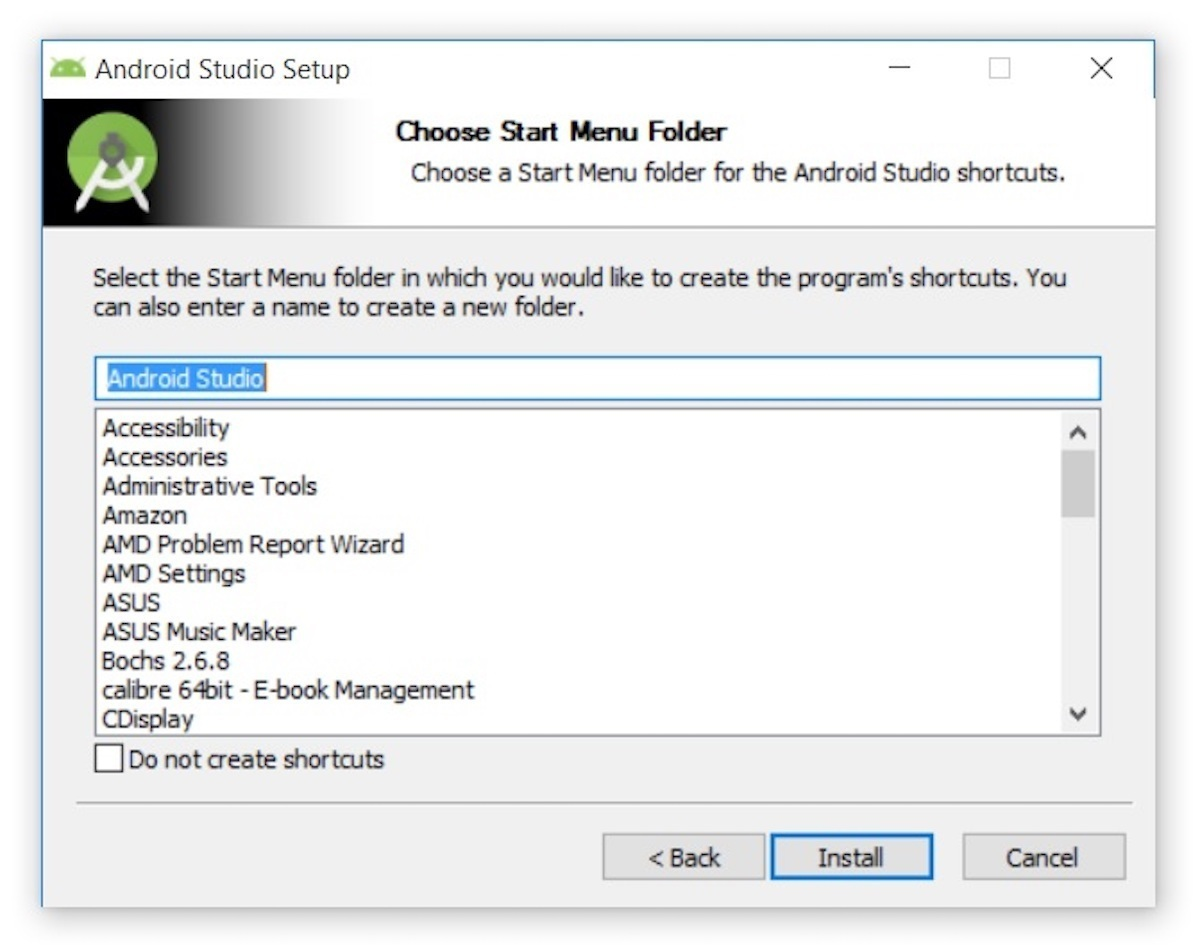
\includegraphics[width=4cm]{figures/installas/4.jpg}
		\centering
		\caption{Membuat shorcut Android Studio.}
	\end{figure}
	\item Kemudian proses instalasi akan berjalan. Show details untuk menampilkan file yang diinstal.
	\begin{figure}[h!]
		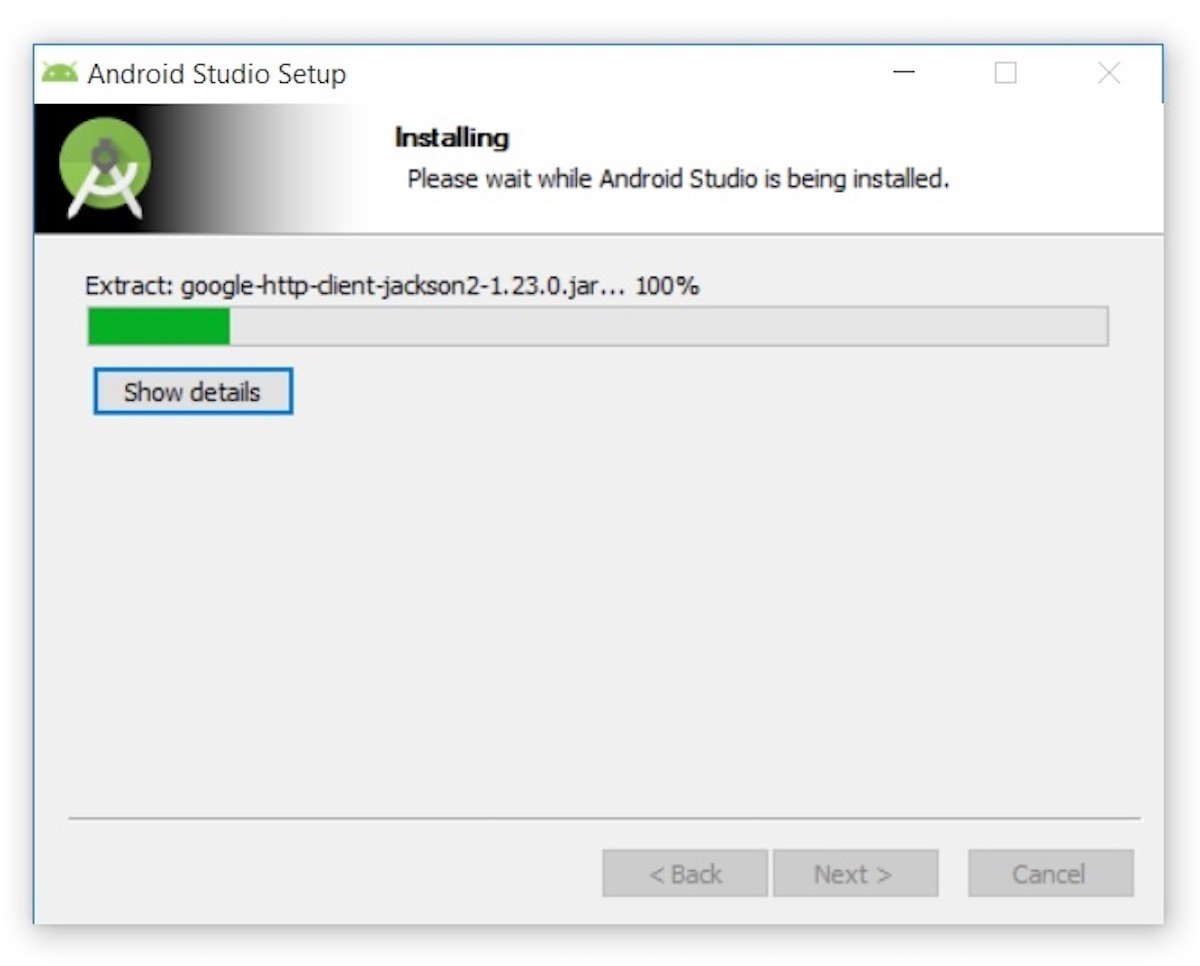
\includegraphics[width=4cm]{figures/installas/5.jpg}
		\centering
		\caption{Proses instalasi.}
	\end{figure}
	\item Setelah proses instal selesai, klik Next.
	\begin{figure}[H]
		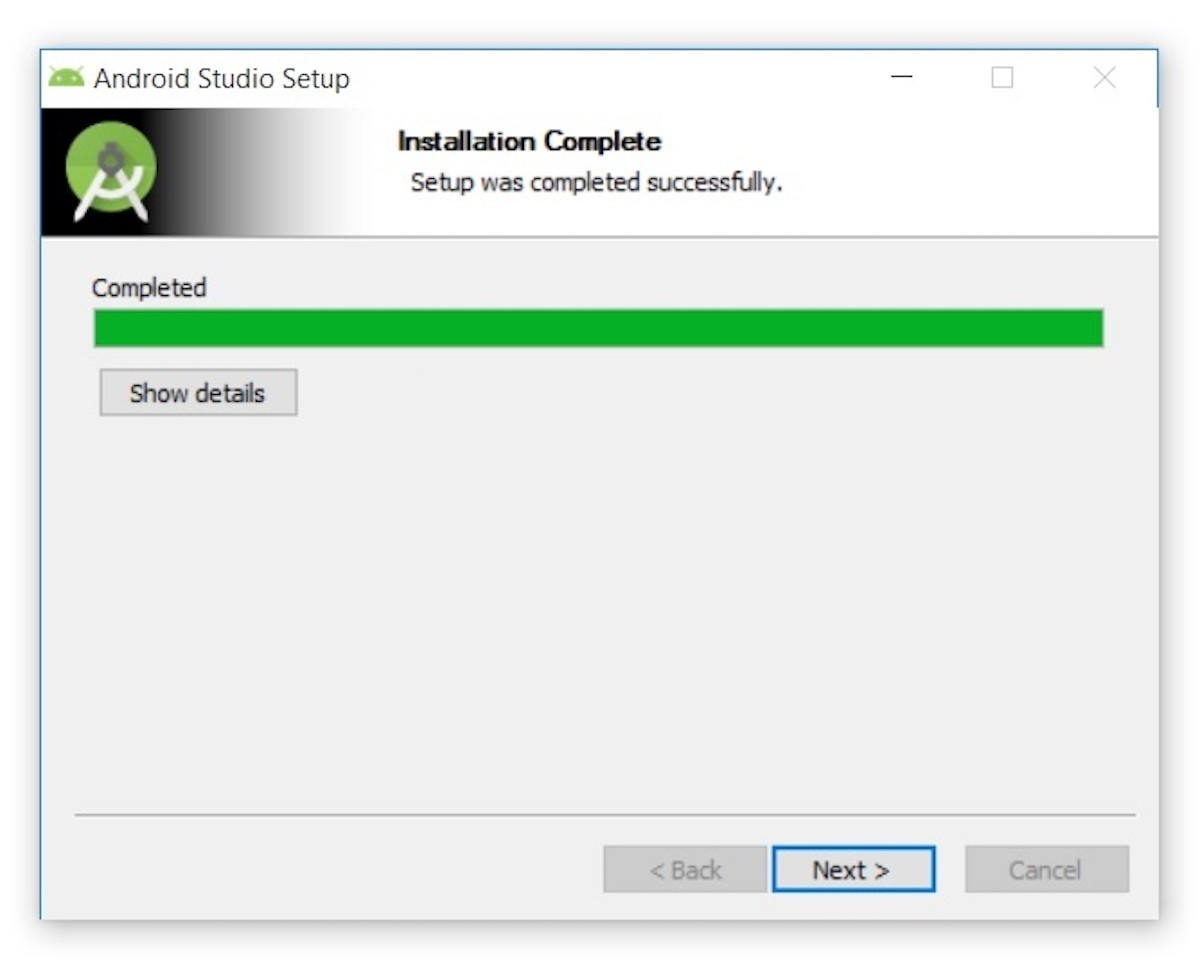
\includegraphics[width=4cm]{figures/installas/6.jpg}
		\centering
		\caption{Proses instalasi selesai.}
	\end{figure}
	\item Kemudian centang Start Android Studio untuk membuka aplikasinya, lalu klik Finish.
	\begin{figure}[H]
		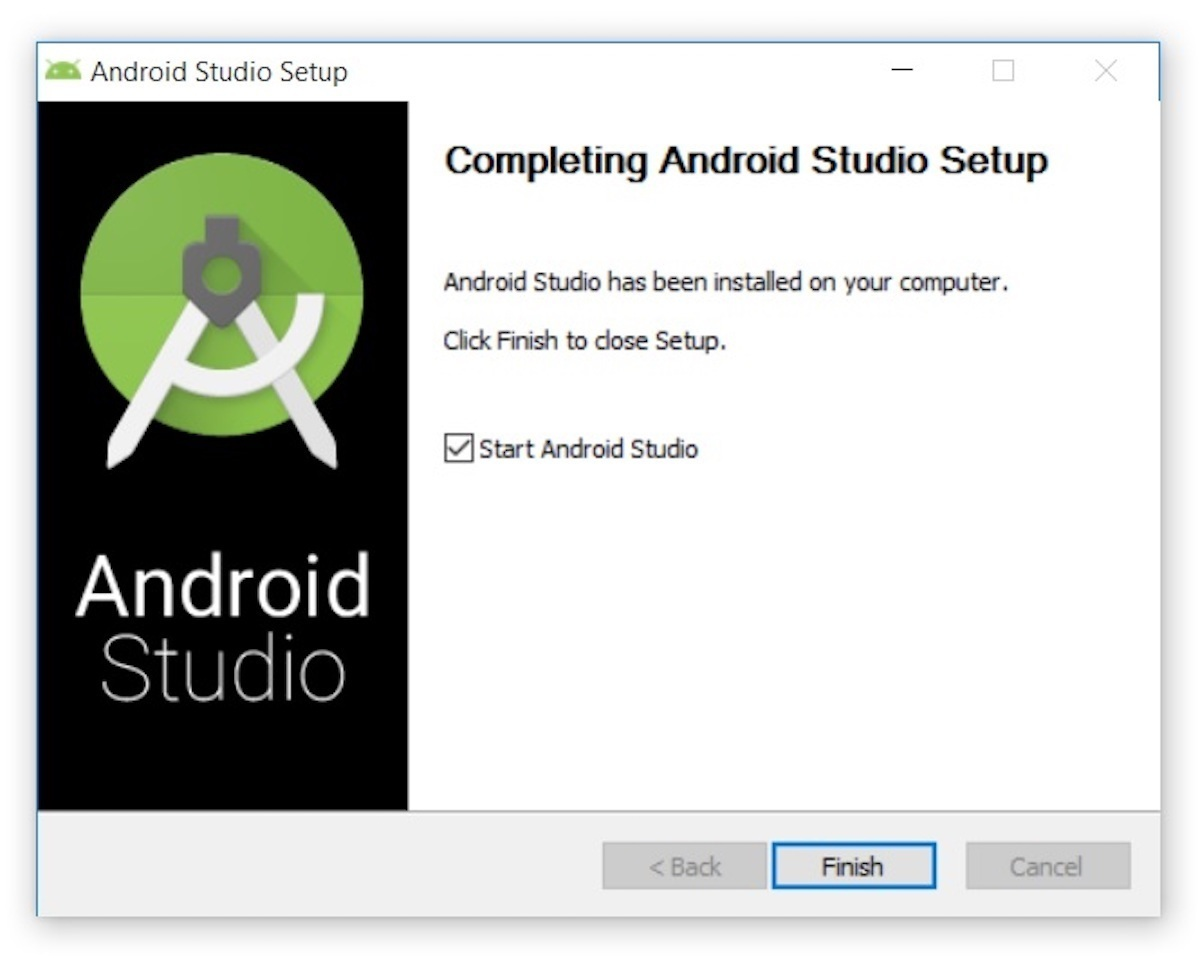
\includegraphics[width=4cm]{figures/installas/7.jpg}
		\centering
		\caption{Jalankan Android Studio.}
	\end{figure}
	\item Ketika Android Studio dijalankan pertama kali, dialog Complete Installation akan muncul dan memberi opsi untuk mengimport setting dari instalasi sebelumnya. Disini kita pilih Do not import settings, lalu klik OK.
	\begin{figure}[H]
		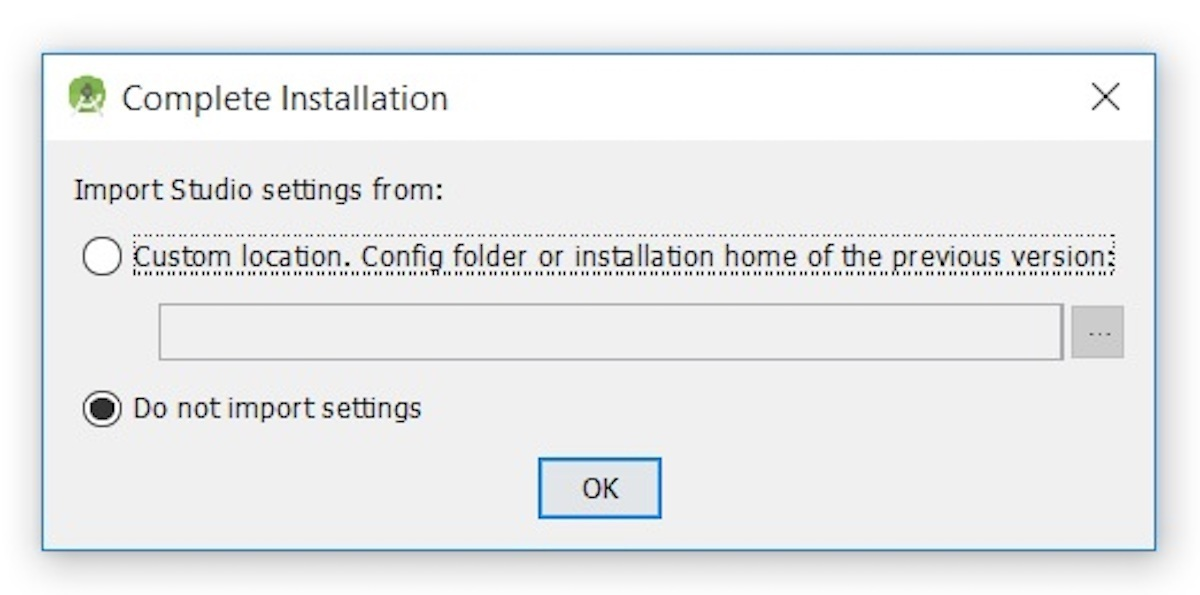
\includegraphics[width=4cm]{figures/installas/8.jpg}
		\centering
		\caption{Import setting instalasi sebelumnya.}
	\end{figure}
	
	\item Kemudian akan muncul splash screen dari Android Studio.
	\begin{figure}[H]
		
\includegraphics[width=4cm]{figures/installas/9.jpg}
		\centering
		\caption{Splash screen Android Studio.}
	\end{figure}
	
	\item Pertama
	\begin{figure}[H]
		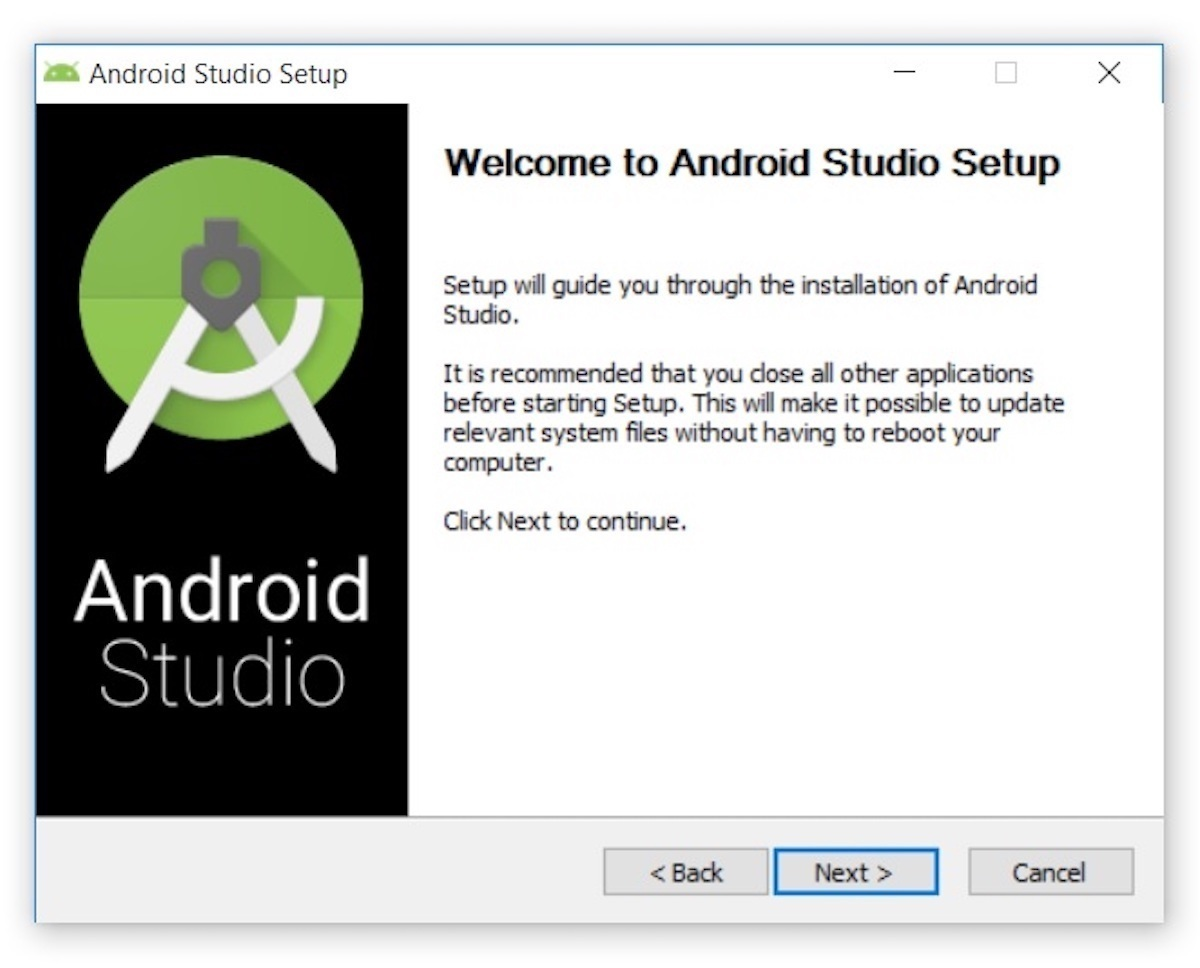
\includegraphics[width=4cm]{figures/installas/1.jpg}
		\centering
		\caption{.}
	\end{figure}
	
	\item Pertama
	\begin{figure}[H]
		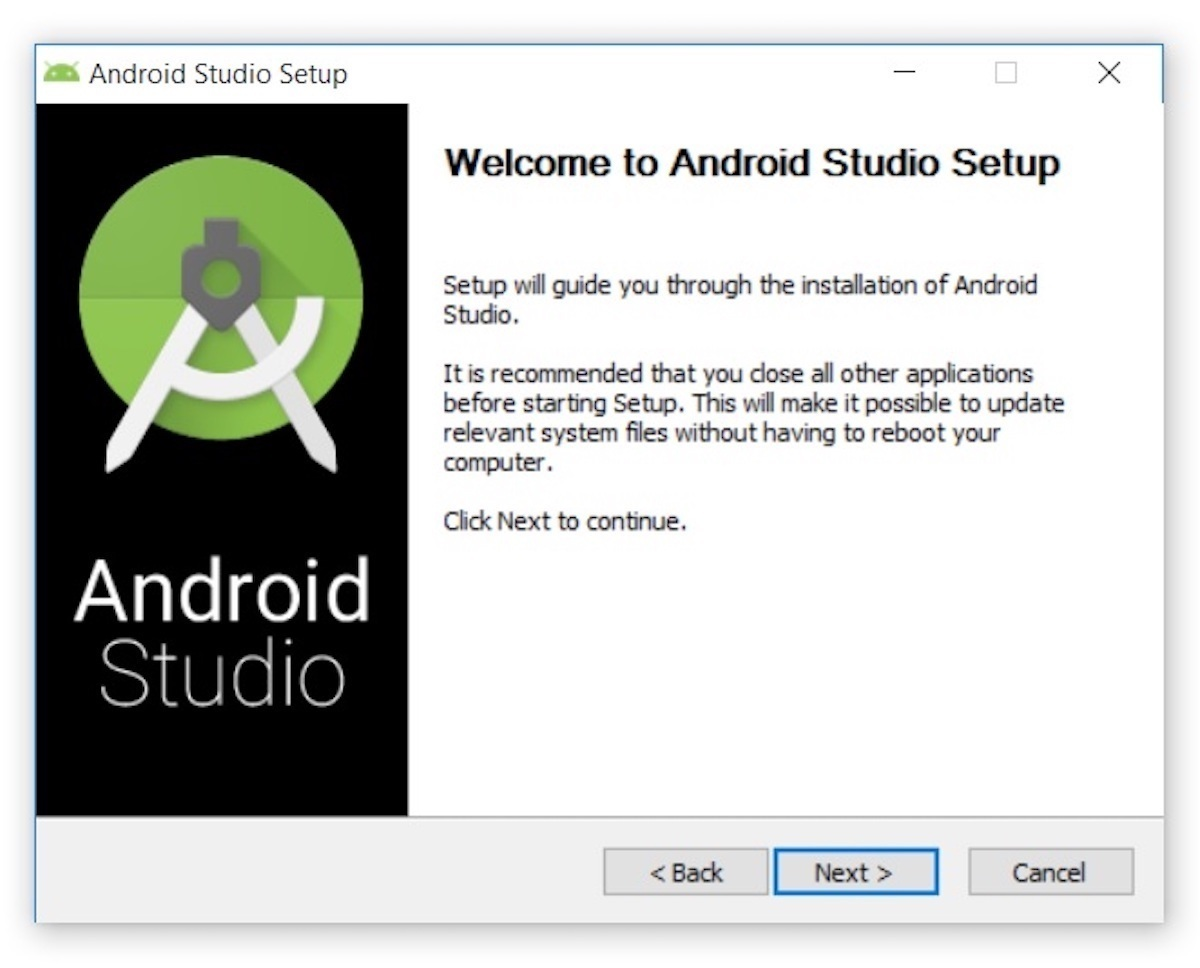
\includegraphics[width=4cm]{figures/installas/1.jpg}
		\centering
		\caption{.}
	\end{figure}
	
	\item Pertama
	\begin{figure}[H]
		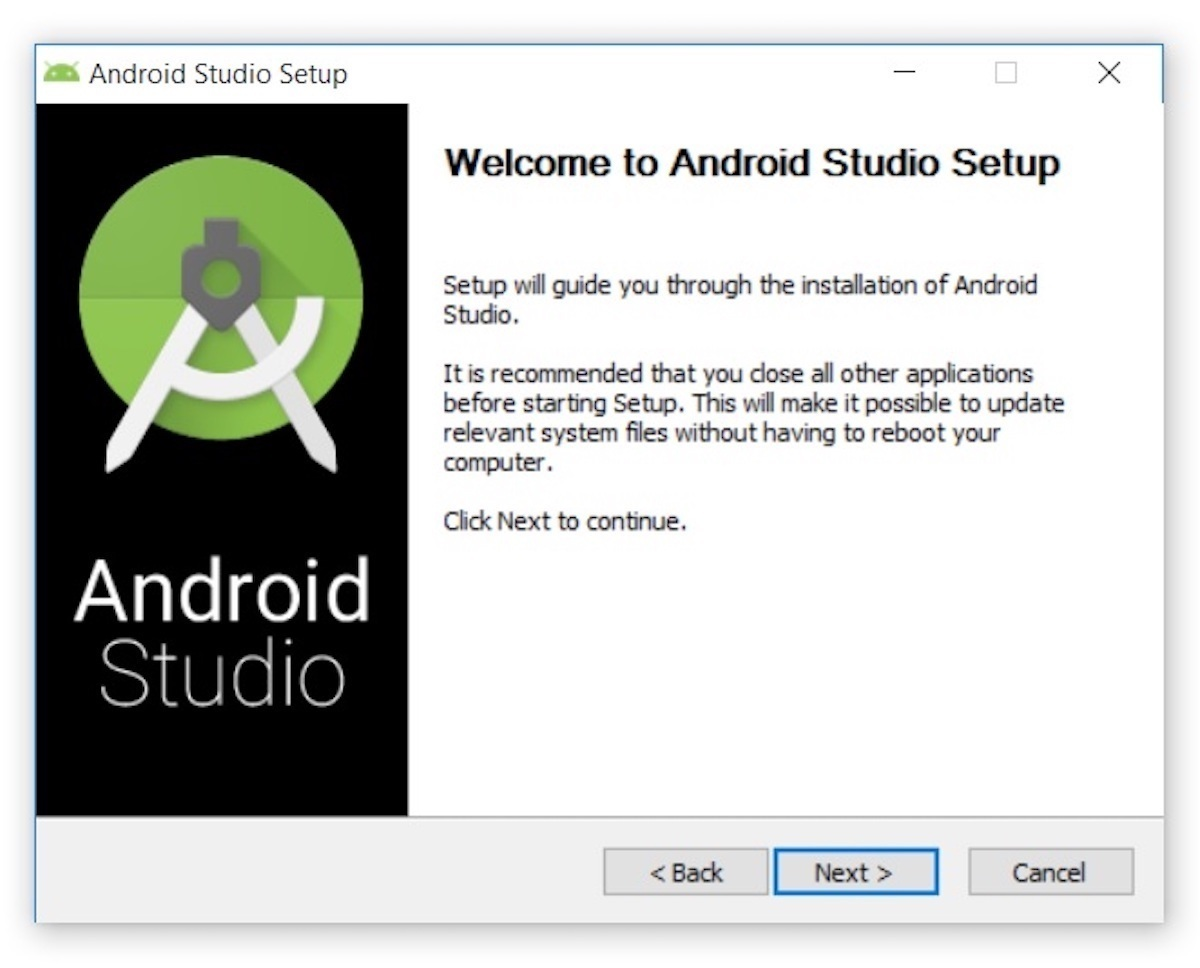
\includegraphics[width=4cm]{figures/installas/1.jpg}
		\centering
		\caption{.}
	\end{figure}
	
	\item Pertama
	\begin{figure}[H]
		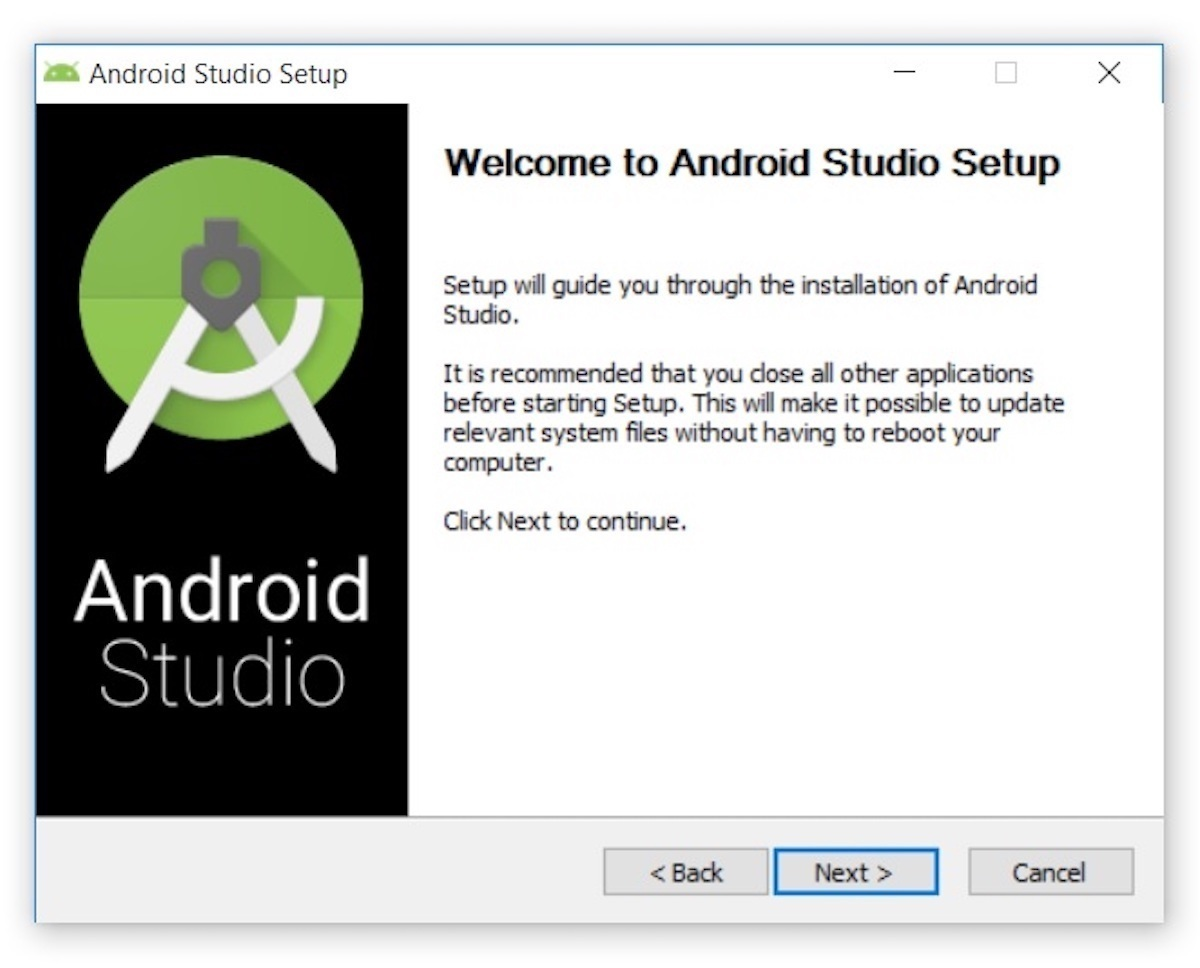
\includegraphics[width=4cm]{figures/installas/1.jpg}
		\centering
		\caption{.}
	\end{figure}
	
	\item Pertama
	\begin{figure}[H]
		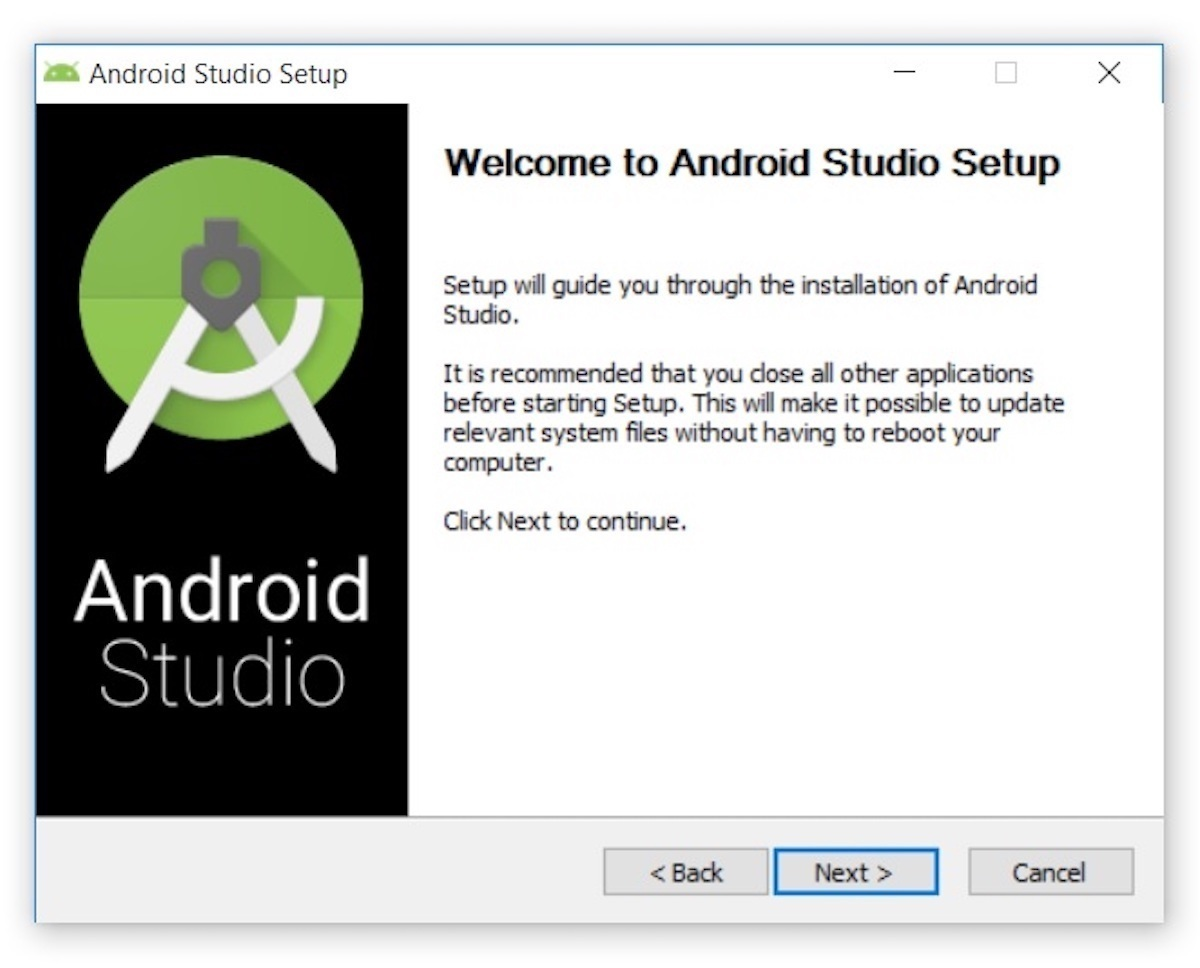
\includegraphics[width=4cm]{figures/installas/1.jpg}
		\centering
		\caption{.}
	\end{figure}
	
	\item Pertama
	\begin{figure}[H]
		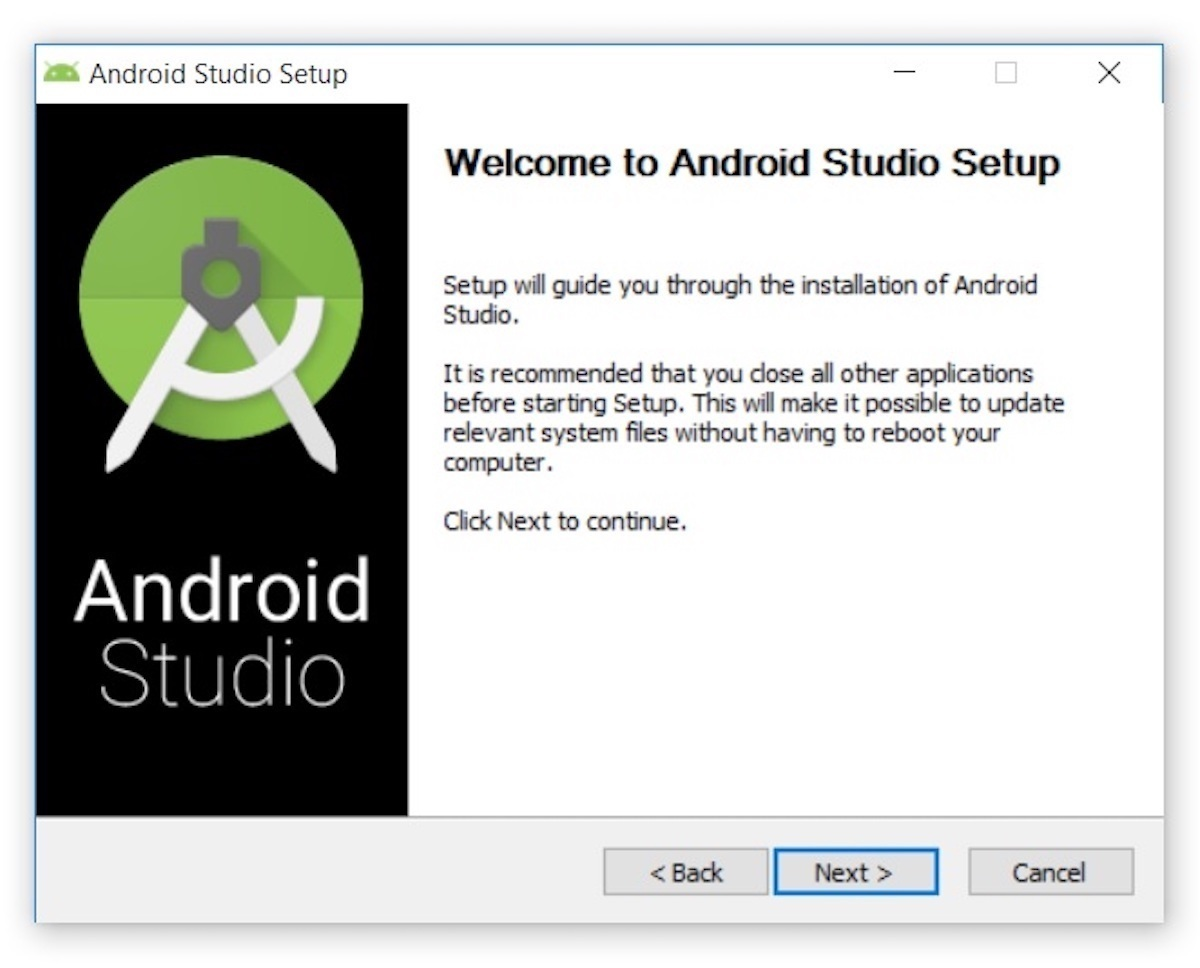
\includegraphics[width=4cm]{figures/installas/1.jpg}
		\centering
		\caption{.}
	\end{figure}
	\begin{figure}[H]
		
\includegraphics[width=4cm]{figures/web/php.png}
		\centering
		\caption{Logo PHP}
	\end{figure}


\subsection{Apa itu PHP?}
PHP adalah bahasa pemrograman yang sering disisipkan ke dalam HTML. PHP memiliki kepanjangan yaitu PHP: Hypertext Preprocessor.Bahasa pemrograman ini menggunakan sistem server-side. Server-side programming adalah jenis bahasa pemrograman yang nantinya script/program tersebut akan dijalankan/diproses oleh server. 

\subsection{Sejarah PHP}
Pada awalnya PHP merupakan kependekan dari Personal Home Page (Situs personal). PHP pertama kali dibuat oleh Rasmus Lerdorf pada tahun 1995. Pada waktu itu PHP masih bernama Form Interpreted (FI), yang wujudnya berupa sekumpulan skrip yang digunakan untuk mengolah data formulir dari web.

Selanjutnya Rasmus merilis kode sumber tersebut untuk umum dan menamakannya PHP/FI. Dengan perilisan kode sumber ini menjadi sumber terbuka, maka banyak pemrogram yang tertarik untuk ikut mengembangkan PHP.

Pada November 1997, dirilis PHP/FI 2.0. Pada rilis ini, interpreter PHP sudah diimplementasikan dalam program C. Dalam rilis ini disertakan juga modul-modul ekstensi yang meningkatkan kemampuan PHP/FI secara signifikan.

Pada tahun 1997, sebuah perusahaan bernama Zend menulis ulang interpreter PHP menjadi lebih bersih, lebih baik, dan lebih cepat. Kemudian pada Juni 1998, perusahaan tersebut merilis interpreter baru untuk PHP dan meresmikan rilis tersebut sebagai PHP 3.0 dan singkatan PHP diubah menjadi akronim berulang PHP: Hypertext Preprocessing.

Pada pertengahan tahun 1999, Zend merilis interpreter PHP baru dan rilis tersebut dikenal dengan PHP 4.0. PHP 4.0 adalah versi PHP yang paling banyak dipakai pada awal abad ke-21. Versi ini banyak dipakai disebabkan kemampuannya untuk membangun aplikasi web kompleks tetapi tetap memiliki kecepatan dan stabilitas yang tinggi.

Pada Juni 2004, Zend merilis PHP 5.0. Dalam versi ini, inti dari interpreter PHP mengalami perubahan besar. Versi ini juga memasukkan model pemrograman berorientasi objek ke dalam PHP untuk menjawab perkembangan bahasa pemrograman ke arah paradigma berorientasi objek. Peladen web bawaan ditambahkan pada versi 5.4 untuk mempermudah pengembang menjalankan kode PHP tanpa menginstal peladen perangkat lunak.

Versi terbaru dan stabil dari bahasa pemograman PHP saat ini adalah versi 7.4.3 yang dirilis pada tanggal 20 Februari 2020

\subsection{Sekilas tentang pembuat PHP : Rasmus Lerdorf}
	\begin{figure}[H]
		
\includegraphics[width=4cm]{figures/web/rasmuslerdorf.jpg}
		\centering
		\caption{Creator PHP Rasmus Lerdorf }
	\end{figure}
Rasmus Lerdorf merupakan seorang programmer yang berasal dari Denmark. Dia membuat dan membantu menginspirasi pengkodean bahasa PHP, terutama pada 2 versi awal yang kemudian dikembangkan secara grup bersama dengan Jim Winstead (Yang membuat blo.gs), Stig Bakken, Shane Caraveo, Andi Gutmans, dan juga Zeev Suraski. sampai sekarang ia terus berkontribusi pada projek.

Lerdorf lahir di pulau disko di daerah Greenland dan kemudian pindah ke Denmark pada awal hidupnya. kelaurganya pindah dari Kanada ke Denmark pada tahun 1980, lalu pindah lagi ke kota King di Ontario pada tahun 1983. Dia lulus dari SMA King City pada tahun 1988, dan pada tahun 1993 lulus dari Universitas Waterloo dengan gelar  Bachelor of Applied Science di bidang teknik desain sistem. Dua juga ikut berkontribusi dalam Apache HTTP Server dan menambahkan clausa Limit pada mSQL DBMS. 

Dari Septermber 2002 sampai November 2009, Lerdorf bekerja di perusahaan Yahoo sebagai Infrastructure Architecture Engineer. Pada tahun 2010 kemudian bergabung ke perusahaan WePay untuk mengembangkan API (Application Programming Interface). dan pada tahun 2011 ia menjadi seorang konsultan untuk beberapa startup. Kemudian pada 22 Februari 2012 ia bergabung dengan Etsy, sebuah website e-commerce yang berfokus pada hal hal vintage. Dan pada tahun 2013, Rasmus bergabung dengan Jelastic sebagai Senior Advisor untuk membantu mereka mengembangkan teknologi baru.

Selain itu Lerdorf juga sering menjadi pembicara dalam konferensi open source di berbagai belahan dunia. Beberapa topik yang sering dia bahas diantaranya adalah security vulnerabilities dan juga tentang PHP.

Pada tahun 2003, ia di beri penghargaan oleh MIT Technology Review sebagai salah satu dari 100 inovator di dunia yang berada dibawah umur 35
\subsection{Website yang menggunakan PHP} 
	\begin{figure}[H]
		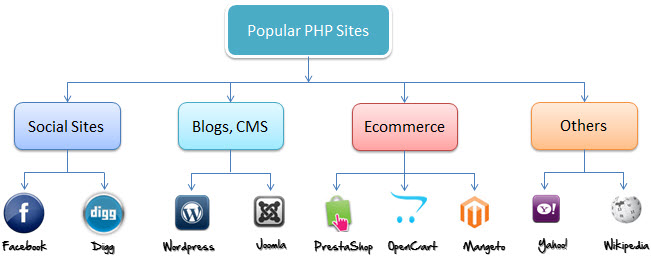
\includegraphics[width=8cm]{figures/web/popularphpsites.jpg}
		\centering
		\caption{Website dengan bahasa PHP}
	\end{figure}

\subsection{Contoh Kode PHP}
	\begin{figure}[H]
		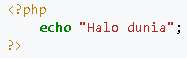
\includegraphics[width=4cm]{figures/web/contohkodingphp.png}
		\centering
		\caption{Program Hello world yang ditulis dengan PHP}
	\end{figure}

\subsection{Kelebihan PHP}
\begin{itemize}
	\item Bahasa pemrograman PHP adalah sebuah bahasa script yang tidak melakukan sebuah kompilasi dalam penggunaannya.
	\item PHP dapat ditemukan di mana - mana
	\item Dalam sisi pengembangan lebih mudah, karena banyaknya developer yang siap membantu dalam pengembangan.
	\item Dalam sisi pemahamanan, PHP adalah bahasa scripting yang paling mudah karena memiliki referensi yang banyak.
	\item PHP adalah bahasa open source yang dapat digunakan di berbagai mesin (Linux, Unix, Macintosh, Windows) dan dapat dijalankan secara runtime melalui console serta juga dapat menjalankan perintah-perintah system
	\item Ringkas
	\item Maintenanace Mudah
\end{itemize}
\subsection{Kekurangan PHP}
\begin{itemize}
	\item Banyak kompetisi, karena PHP adalah bahasa pemrograman yang paling umum
	\item Terkesan kurang prestigious
	\item Tidak ideal jika untuk pengembangan skala besar.
	\item Tidak dapat memisahkan antara tampilan dengan logik dengan baik (Meskipun penggunaan template bisa memperbaikinya)
	\item PHP mempunyai kelemahan security tertentu yang mana jika programmer tidak jeli dalam melakukan pemrograman dan kurang memperhatikan isu dan konfigurasi PHP
\end{itemize}

	\begin{figure}[H]
		
\includegraphics[width=4cm]{figures/web/logocodeigniter.png}
		\centering
		\caption{Logo Codeigniter}
	\end{figure}

\subsection{Pengenalan Codeigniter}

CodeIgniter merupakan aplikasi sumber terbuka yang berupa kerangka kerja PHP dengan model MVC (Model, View, Controller) untuk membangun situs web dinamis dengan menggunakan PHP. CodeIgniter memudahkan pengembang web untuk membuat aplikasi web dengan cepat dan mudah dibandingkan dengan membuatnya dari awal. CodeIgniter dirilis pertama kali pada 28 Februari 2006. Versi stabil terakhir adalah versi 3.1.11
	\begin{figure}[H]
		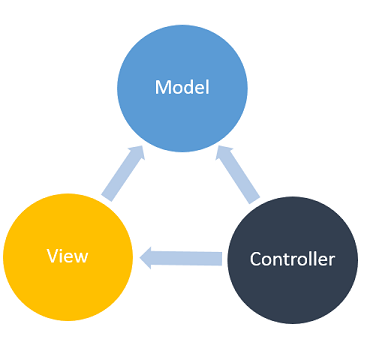
\includegraphics[width=4cm]{figures/web/mvc.png}
		\centering
		\caption{MVC Concept}
	\end{figure}
\subsection{Konsep MVC (Model View dan Controller)}
Model View Controller merupakan suatu konsep yang cukup populer dalam pembangunan aplikasi web, berawal pada bahasa pemrograman Small Talk, MVC memisahkan pengembangan aplikasi berdasarkan komponen utama yang membangun sebuah aplikasi seperti manipulasi data, antarmuka pengguna, dan bagian yang menjadi kontrol aplikasi. Terdapat 3 jenis komponen yang membangun suatu pola MVC dalam suatu aplikasi yaitu: 
\begin{enumerate}
	\item View, merupakan bagian yang menangani logika presentasi. Pada suatu aplikasi web bagian ini biasanya berupa berkas templat HTML, yang diatur oleh controller. View berfungsi untuk menerima dan merepresentasikan data kepada pengguna. Bagian ini tidak memiliki akses langsung terhadap bagian model.
	\item Model, biasanya berhubungan langsung dengan pangkalan data untuk memanipulasi data (insert, update, delete, search), menangani validasi dari bagian controller, tetapi tidak dapat berhubungan langsung dengan bagian view.
	\item Controller, merupakan bagian yang mengatur hubungan antara bagian model dan bagian view, controller berfungsi untuk menerima permintaan dan data dari pengguna kemudian menentukan apa yang akan diproses oleh aplikasi.
\end{enumerate}

\subsection{Kelebihan dan Kekurangan Codeigniter}
\begin{itemize}
	\item Kelebihan
\begin{itemize}
	\item Performa sangat cepat: salah satu alasan tidak menggunakan kerangka kerja adalah karena eksekusinya yang lebih lambat daripada PHP from the scracth, tapi CodeIgniter sangat cepat bahkan mungkin bisa dibilang CodeIgniter merupakan kerangka kerja yang paling cepat dibanding kerangka kerja yang lain
	\item Konfigurasi yang sangat minim
	\item Banyak komunitas: dengan banyaknya komunitas CI ini, memudahkan kita untuk berinteraksi dengan yang lain, baik itu bertanya atau teknologi terbaru
	\item Dokumentasi yang sangat lengkap
\end{itemize}
	\item Kekurangan
\begin{itemize}
	\item CodeIgniter tidak ditujukan untuk pembuatan web dengan skala besar.
	\item Library yang sangat terbatas.
	\item Tidak Adanya Editor Khusus.
\end{itemize}
\end{itemize}
\subsection{Instalasi Codeigniter}


\end{enumerate}


\bibliographystyle{IEEEtran} 
%\def\bibfont{\normalsize}
\bibliography{references}


%%%%%%%%%%%%%%%
%%  The default LaTeX Index
%%  Don't need to add any commands before \begin{document}
\printindex

%%%% Making an index
%% 
%% 1. Make index entries, don't leave any spaces so that they
%% will be sorted correctly.
%% 
%% \index{term}
%% \index{term!subterm}
%% \index{term!subterm!subsubterm}
%% 
%% 2. Run LaTeX several times to produce <filename>.idx
%% 
%% 3. On command line, type  makeindx <filename> which
%% will produce <filename>.ind 
%% 
%% 4. Type \printindex to make the index appear in your book.
%% 
%% 5. If you would like to edit <filename>.ind 
%% you may do so. See docs.pdf for more information.
%% 
%%%%%%%%%%%%%%%%%%%%%%%%%%%%%%

%%%%%%%%%%%%%% Making Multiple Indices %%%%%%%%%%%%%%%%
%% 1. 
%% \usepackage{multind}
%% \makeindex{book}
%% \makeindex{authors}
%% \begin{document}
%% 
%% 2.
%% % add index terms to your book, ie,
%% \index{book}{A term to go to the topic index}
%% \index{authors}{Put this author in the author index}
%% 
%% \index{book}{Cows}
%% \index{book}{Cows!Jersey}
%% \index{book}{Cows!Jersey!Brown}
%% 
%% \index{author}{Douglas Adams}
%% \index{author}{Boethius}
%% \index{author}{Mark Twain}
%% 
%% 3. On command line type 
%% makeindex topic 
%% makeindex authors
%% 
%% 4.
%% this is a Wiley command to make the indices print:
%% \multiprintindex{book}{Topic index}
%% \multiprintindex{authors}{Author index}

\end{document}


